\documentclass[11pt]{article}
\usepackage[utf8]{inputenc}
\usepackage{graphicx}
\date{}
\usepackage{amssymb}
\usepackage{amsmath}
\usepackage{float}
\usepackage{subfig}

\usepackage{apacite}
\usepackage{listings}
\lstdefinestyle{myCustomCStyle}{
  language=C,
  numbers=left,
  stepnumber=1,
  numbersep=10pt,
  tabsize=4,
  showspaces=false,
  showstringspaces=false
}
\renewcommand{\lstlistingname}{Algorithm}% Listing -> Algorithm
\renewcommand{\lstlistlistingname}{List of \lstlistingname s}
\usepackage{listings}
\usepackage{xcolor} % for setting colors

% set the default code style
\lstset{
    frame=tb, % draw a frame at the top and bottom of the code block
    tabsize=4, % tab space width
    showstringspaces=false, % don't mark spaces in strings
    numbers=left, % display line numbers on the left
    commentstyle=\color{green}, % comment color
    keywordstyle=\color{blue}, % keyword color
    stringstyle=\color{red} % string color
}



\usepackage[margin=1.5in]{geometry}
\usepackage[english]{babel}
\usepackage[utf8]{inputenc}
\usepackage{algorithm}
\usepackage[noend]{algpseudocode}
\usepackage{amsfonts}
\usepackage{titlesec}
\begin{document}
\title{\line(1,0){250} \\ \huge{\textbf{2019-2020 Bahar Yarıyılı \\ BLM2512 Veri Yapıları ve Algoritmalar Dönem Projesi}} \\\line(1,0){250}}
\author{\textsc{Mesut Şafak Bilici} \\ 17011086}
\maketitle
\tableofcontents
\hspace*{-0.6cm}\textbf{5} \; \textbf{Kod} \hspace*{12.3cm}\textbf{10}

\pagebreak
\section{Çalıştırmadan Önce..}
\hspace*{1cm} input-3.txt isimli dosyanın okunması, node sayısının bulunması, graph'ın oluşturulması ve BFS algoritmasının uygulanması toplamda 14 dakikayı bulmaktadır.\\
İstenilen ismin connection map'ini bulmak için ismi "Soyisim, İsim"
şeklinde girmeniz gerekmektedir.
\section{Yöntem}
\hspace*{1cm} İstenilen algoritma farklı bölümlere sahiptir. Öncelikle, verilen veriyi graph'a dökmek için graph'ımızın vertex sayısını bilmemiz gerekmektedir. Verilen film-oyuncu verisi\\
\hspace*{2cm} $\rightarrow$ film1/soyad-actor1, isim-actor1/soyad-actor2, isim-actor2\\
\hspace*{2cm} $\rightarrow$ film2/soyad-actor2, isim-actor2/ $\dots$\\
şeklinde verildiği için, stringler üzerinde bir tokenize işlemi yapmamız gerekli. Bu tokenize işlemi ise, her satırda ilk önce '\textbackslash n' karakterini ayrıştırarak daha sonra ise '/' karakterini ayrıştırarak yapılmalıdır. Bu sayede verimizdeki film ve kaç aktör sayısı tokenize işlemi sayısına eşit olacaktır. Fakat bir aktör birden fazla filmde oynamış olabilir. Bu ise yapacağımız işlemi değiştirecektir. Birden fazla filmde oynayan aktörleri tek bir kişi saymamız için her satırın birleşim kümesini bulmamız gerekmektedir. Bu sayede graph'ımızın vertex sayısını bulabiliriz. Vertex sayımızı bulduktan sonra her aktörü ve filmi bir node haline getirip graph'ımızı oluşturuyoruz. Daha sonra ise Breadth First Search ile her aktör vertex'inin Kevin Bacon'a olan uzaklığını buluyoruz. Bu Breadth First Search işlemini yaparken her vertex'in parent'ını tutmak, istenilen karakterin Kevin Bacon ile arasında olan connection map'i göstermemiz için (izlediği en kısa yol) işimize yarayacaktır. Aşağıda bu yapılan işlemlerin her biri ayrı fonksiyon ve değişken başlıkları altında örnekleri verilerek daha detaylı açıklanacaktır ve bazı oyuncular için çıktılar gösterilecektir.
\section{Algoritma: Değişkenler ve Fonksiyonlar}
Bu kısımda her bir işlem için gerekli olan değişkenler ve algoritmalar açıklanacaktır. Toplamda 3 ayrı struct, 13 tane fonksiyon, 2 tane global dizi kullanılmıştır.
\subsection{Global Değişkenler}
\hspace*{1cm} Kod boyunca neredeyse her yerde kullanılacak 2 farkı dizi global değişken olarak tanımlanmıştır. Bu dizilerin isimleri ile beraber, yaptığı işler aşağıda açıklanmıştır:
\begin{itemize}
	\item \textbf{char} \textsf{storage[190000][300]:} Bu değişkeni vertex sayımızı hesaplamak için ve aynı zamanda her bir film/aktör vertex'ine belirli bir $i$ $\in$ $\mathbb{N}$ index'ini atamak için tanımladık. Kullanıldığı fonksiyonlar içinde yaptığı iş daha detaylı şekilde açıklanacaktır.
	\item \textbf{int} \textsf{int moviectrl[190000]:} Vertex sayısını hesaplarken gelen verinin film mi yoksa aktör mü olduğu bilgisini tutmakta belirlenmiştir. Boolean değerler tutan bir dizidir. Eğer film ise 1, aktör ise 1 tutmaktadır. Her bir index \textsf{storage} dizisinin indexine karşılık gelmektedir. Yani \textsf{storage[$k$]} içindeki film/aktör ismi'nin film mi yoksa aktör mü olduğu bilgisi \textsf{moviectrl[$k$]} içinde saklanmaktadır.
\end{itemize}
\subsection{Fonksiyonlar}
\hspace*{1cm} Kod boyunca toplamda 13 ayrı fonksiyon kullanılmıştır. Bunlardan 4'ü graph yapısını oluşturmak için, 3'ü Breadth First Search için, 2'si Kevin Bacon frekans dizisini oluşturmak için, 1'i en kısa yolu bulmak için, 2 tanesi önceden hesaplanmış yolu bastırmak için, son 1 tanesi ise opsiyonel olarak graph yapısını bastırmak için.

\begin{itemize}

	\item \textbf{int} \textsf{numberOfVertex(FILE*):} Algoritma, elimizdeki veriyi okuyup tokenize ederek kaç aktör ve kaç film olduğunu bulmaktadır. Veride her film isminden 1 tane olmasına rağmen herhangi bir aktör 2 veya 2'den fazla filmde oynayabilir. Bunu kontrol etmezsek aynı aktöre ait 2 farklı node açmış oluruz. Algoritmada ilk önce satır satır verimizi okumaya başlıyoruz ve ilk önce '\textbackslash n' karakterini elimizdeki satırdan ayrıştırıyoruz. Sonra ise ayrıştıracak bir string kalmayana kadar '/' karakterini ayrıştırıyoruz. Teker teker bu film-aktör isimlerini \textsf{storage} dizisine yerleştiriyoruz, fakat bunu yaparken en baştan \textsf{storage} dizisini kontrol ediyoruz. Eğer hiçbir elemanı elimize gelen aktör stringine denk değilse bu elemanı \textsf{storage} dizisinin son elemanından bir sonraki elemana atıyoruz. Elimizdeki dosya'nın sonu gelene kadar bunu yapıyoruz. Bu işlem bittikten sonra artık \textsf{storage} dizisi elimizdeki her filmi-aktörü bulunduruyor olacak. İşimiz kolaylaşsın diye, her bir film-aktör'ün vertex numarasını da \textsf{storage} içindeki index adresi belirliyoruz.
	
	\item  \textbf{NODE*} \textsf{createNode(int,char*):} Gelen her elemanı linked list'in başına ekleyen fonksiyondur. Bunu yaparken hangi vertex olduğu ve hangi isimli film-aktör olduğu verilerini de atamaktadır.
	\item \textbf{GRAPH*} \textsf{createGraph(int):} vertex sayısı $\times$ NODE struct'ı boyutunda bir linked list dizisi açmaktadır. Graph yapısı burada tutulacaktır. Bu dizinin ismi adjList[]'dir.
	
	\item \textbf{GRAPH*} \textsf{addEdge(int,char*):} Bu fonksiyonda hangi aktör hangi film ile bağlantılı olacağını hesaplıyoruz. Bunu yaparken yine dosyayı okuyoruz, string tokenizer ile ayrıştırarak. Bu sefer elimize gelen her yeni stringi \textsf{storage} dizisinin elemanları ile karşılaştırıyoruz.  Doğal olarak bu dizinin içinde bir yerlerde bu film-aktör ismi olmak zorunda. \textsf{storage} isimli dizinin içinde elimize gelen yeni stringi bulduğumuzda bu string'in bulunduğu index'i bulmak istriyoruz aslında. Bundan sonra bu index'e sahip bir node yaratıyoruz $createNode()$ fonksiyonu ile ve bu node'u satır başında hangi film varsa onunla bağlıyoruz (edge oluşturuyoruz). Bu şu anlama gelmekterdir: $\forall$ $k$ $\in$ $\mathbb{N}$ için adjList[k]'daki node'lar \textsf{storage[$k$]}'daki verinin bağlantılarıdır. Adımları daha açıklayıcı göstermek için pseudo-code aşağıdaki gibidir: \\
\\
\\
\\
\\
\begin{algorithm}
\caption{addEdge}
\begin{algorithmic}[1]

    \State Vertex sayısı kadar adjList[] dizisi yarat.
    \State $j$ $\leftarrow$ Her satır başındaki filmin \textsf{storage} içindeki index'ini bul.
    \State $i$ $\leftarrow$ Text dosyasından gelen her aktörün \textsf{storage} içindeki index'ini bul. 
    
    \State $i$ değeri ile node yarat ve adjList[j]'e ekle. 
    \State $j$ değeri ile node yarat ve adjList[i]'e ekle
\end{algorithmic}
\end{algorithm}\\
Aynı zamanda bu işlemlerin her biri yapılırken file içindeki her satır tokenize edilirken, ilk tokenize edilen cümleyi yani film isminin karşılık geldiği $k$ indexini moviectrl isimli integer/boolean dizisinin $k$ indexini 1 yaptım.\\ 
Şöyle açıklarsak daha anlaşılır olacaktır, elimde bir veri var ve bu verinin storage isimli dizideki index'i $k$ olsun. Eğer bu veri herhangi bir satırda ilk tokenize edilen cümle ise filmdir, değilse aktördür. Daha sonra ise yine aynı $k$ indexine karşılık gelecek şekilde \textsf{moviectrl[$k$]} bölmesi filmse 1, aktörse 0 yapılır. Bu kontrol ilerde Bacon numarası için frekans hesaplaması yaparken işimize yarayacaktır.
\item \textbf{void} \textsf{printGraph(GRAPH*,int):}
\begin{figure}[H]
\centering
\includegraphics[width=15cm]{image1.png}
\caption{Graph'ın bir kısmının ekran görüntüsü.}
\label{fig:figure3}
\end{figure}
Graph'ın bastırılması şu şekilde olmuştur:\\
storage[i](vertex i): graph-$>$adjList[j](vertex m) / graph- $>$adjList[j]-$>$next(vertex n)\\
storage[m](vertex m): graph-$>$adjList[k](vertex i)\\
storage[n](vertex n): graph-$>$adjList[p](vertex i)\\

	\item \textbf{void} \textsf{eunqueue(QUEUE**,int,char*):} Queue'ya eleman eklediğimiz fonksiyon. Ek olarak Queue'ya node atarken graph node'unun vertex numarasını ve film-aktör verisini de Queue noduna atıyoruz.

	\item \textbf{QUEUE*} \textsf{dequeue(QUEUE**):} Queue'dan eleman çektiğimiz fonksiyon. Ek olarak Queue boş olduğunda fonksiyon NULL döndürüyor.
\\
	\item \textbf{void} \textsf{BreadthFirstSearch(GRAPH**,char*,int,int*,int*):} Breadth First Search bipartite graph'ta enine arama yapılmak üzere kullanılmıştır. Her node'un (filmler dahil) Kevin Bacon'a olan \textit{en kısa} uzunluğu hesaplanacaktır. Bunu yaparken yukarıda açıklanan \textsf{enqueue} ve \textsf{dequeue} fonksiyonları ile birlikte Queue yapısı kullanılmıştır.
Breadth First Search yaparken ilk önce "Bacon, Kevin" node'unun hangi index'te, diğer bir sözle, "Bacon, Kevin" isminin hang \textsf{storage[]} index'inde olduğu hesaplanmıştır.
\begin{figure}[H]
\centering
\includegraphics[width=3cm]{graph.png}
\caption{Örnek graf modeli.}
\label{fig:figure3}
\end{figure}
Algoritmanın nasıl çalıştığını Figure 2'den ilerleyerek gösterelim. 0 index'li node'un "Kevin Bacon" node'u olduğunu varsayalım (başlangıç node'u Kevin Bacon olmayan senaryolar da olabilir). İlk önce \textsf{visited} isimli Kevin Bacon'a olan uzaklıkları tutan integer dizimizin tüm elemanlarını -1 yapıyoruz. Bu sayede asla ulaşamadığımız node'ların uzaklık değeri -1 oluyor.\\
Kevin Bacon'dan başlıyoruz ve Kevin Bacon'ı queue yapısına atıyoruz. Daha sonra queue'dan son elemanı çekip komşularına, yani 2 4 5 node'larını, geziyoruz. 2 4 5 node'larının ancak ve ancak film olabileceğini belirtelim. Bu node'ları gezerken sırasıyla 2 4 5 node'larını da queue'ya atıyoruz. Bu node'ların visited sayısı parentlarının visited sayısı oluyor. Bu gezme işlemini yaparken \textsf{parent} isimli arrayin içinde gezdiğimiz node'ların bir üst node'unu yani parentının da indexini tutuyoruz. Bu işlem yolu bastırırken işimize yarayacak.\\
Sonra queue'ya attığımız ilk elemanı çekiyoruz yani 2 numaralı node'u. Sonrasında komşusu olan 3'ü, 3 bir aktör, gezmiş oluyoruz. Bu işlem bu şekilde devam ediyor. Komşu kalmadığını anlamamız için dequeue işlemi yapılırken çekecek eleman kalmadığında NULL döndürüyoruz. Artık elimizde parent ve visited dizileri var.

	\item \textbf{void} \textsf{findMaxDistance(int,int*):} Frekans dizimizin bir boyunun olması zorunlu. Histogram mantığı ile bir frekans dizisi oluşturacağımızdan visited dizisinin en büyük elemanı frekans dizimizin eleman sayısı olarak seçiliyor. Aynı zamanda bu işlem yapılmadan önce her visited değerine 2 ile bölünmüş hali atanıyor. Çünkü \\
	\hspace*{3cm}film1 - oyuncu1 - film2 - oyuncu2\\
gibi bir arama yapıldığında oyuncu 1 ile oyuncu 2 arasındaki mesafe 2 çıkmaktadır çünkü aradaki filmi de sayıyoruz.
	\item \textbf{int*} \textsf{frequencyListOfKevinBaconNumbers(GRAPH*,int,int,int*):} Eğer moviectrl arrayındaki bilgi 0 ise, yani aktör ise, $ i \in nvertices$(graph) olacak şekilde $frequency[visited[i]] = frequency[visited[i]] + 1$ işlemi yapılıyor. 0 değeri sonsuz olarak sayılmıştır fakat bastırılırken sonsuz kelimesi yazılmıştır. Kevin Bacon'ın da sayısı sıfır olarak atanmıştır ama sonsuz frekansından bir çıkartılarak özel olarak Kevin Bacon'ın Kevin Bacon sayısı gösterilmiştir.
	\item \textbf{void} \textsf{shortestDistance(GRAPH*,char*,int,int*,int*,char*):} Kimin Kevin Bacon ile olan bağlantısını bulmak istiyorsak o kişinin \textsf{storage} arrayindeki index'ini buluyoruz. Bundan sonra yapılacak işlem zaten aslında \textsf{BreadthFirstSearch} fonksiyonu içinde yapılmıştı. Parent tutmak. Figure 2'de görüldüğü gibi 6 numaralı node'a ulaşıldığında 6'nın parent'ı 3 numaralı node, 3'ün parent'ı 2, 2'nin parent'ı ise 0. Bunu index'lerle göstermek gerekirse:\\ \\
	\hspace*{2cm}parent[6] = 3\\
	\hspace*{2cm}parent[parent[6]] = 2\\
	\hspace*{2cm}parent[parent[parent[6]]] = 0\\\\
olacaktır. Her bir parent'ı \textsf{path} isimli bir arrayin içinde tutup, path dizisi bastırılmıştır. Parent'lar film-aktör-film-aktör... şeklinde ilerleyeceği için bastırma işlemi $\forall i \in n(path)$:\\\\
	\hspace*{2cm} path[i] (aktör)\\
	\hspace*{2cm} path[i+2] (film)\\
	\hspace*{2cm} path[i+1] (aktör)\\\\
şeklinde $i=i+2$ index arttırılması ile gerçekleşmektedir.
\\Ayrıca bu fonkisyon içinde projede bonus olarak bahsedilen işlem gerçekleşmektedir. Eğer önceden istenilen ismin yolu hesaplandıysa LL isimli structa ait olan linked list'ten bu ismin yolu alınır. Eğer yoksa hesaplanır ve hesaplandıktan sonra linked list'e yeni isim koyulur. Tekrardan o isim hesaplanmak istediğinde bu sefer linked list'teki önceden hesaplanmış yol basılır.
\end{itemize}
\section{İstenilen Çıktılar}
Adile Naşit'in ismi verilen input-3 datasında olmadığı için girilen isim verilen data içinde değildir uyarısı vermektedir.

\begin{figure}[H]
\centering
\includegraphics[width=13cm]{son.png}
\caption{İstenilen çıktılar.}
\label{fig:figure3}
\end{figure}

\begin{figure}[H]
\centering

\includegraphics[width=14cm]{1.png}
\caption{input-2.txt'den Pitt, Brad.}
\label{fig:figure3}
\end{figure}
\begin{figure}[H]
\centering
\includegraphics[width=14cm]{2.png}
\caption{input-2.txt Dix, Richard.}
\label{fig:figure3}
\end{figure}
\begin{figure}[H]
\centering
\includegraphics[width=14cm]{3.png}
\caption{input-2.txt'den Corcoran, Hugh.}
\label{fig:figure3}
\end{figure}
\begin{figure}[H]
\centering
\includegraphics[width=14cm]{4.png}
\caption{input-2.txt'den Barrows, Dan.}
\label{fig:figure3}
\end{figure}
\begin{figure}[H]
\centering
\includegraphics[width=14cm]{5.png}
\caption{input-2.txt'den Blue, Monte.}
\label{fig:figure3}
\end{figure}
\begin{figure}[H]
\centering
\includegraphics[width=14cm]{6.png}
\caption{input-2.txt'den Call, Edward.}
\label{fig:figure3}
\end{figure}
\begin{figure}[H]
\centering
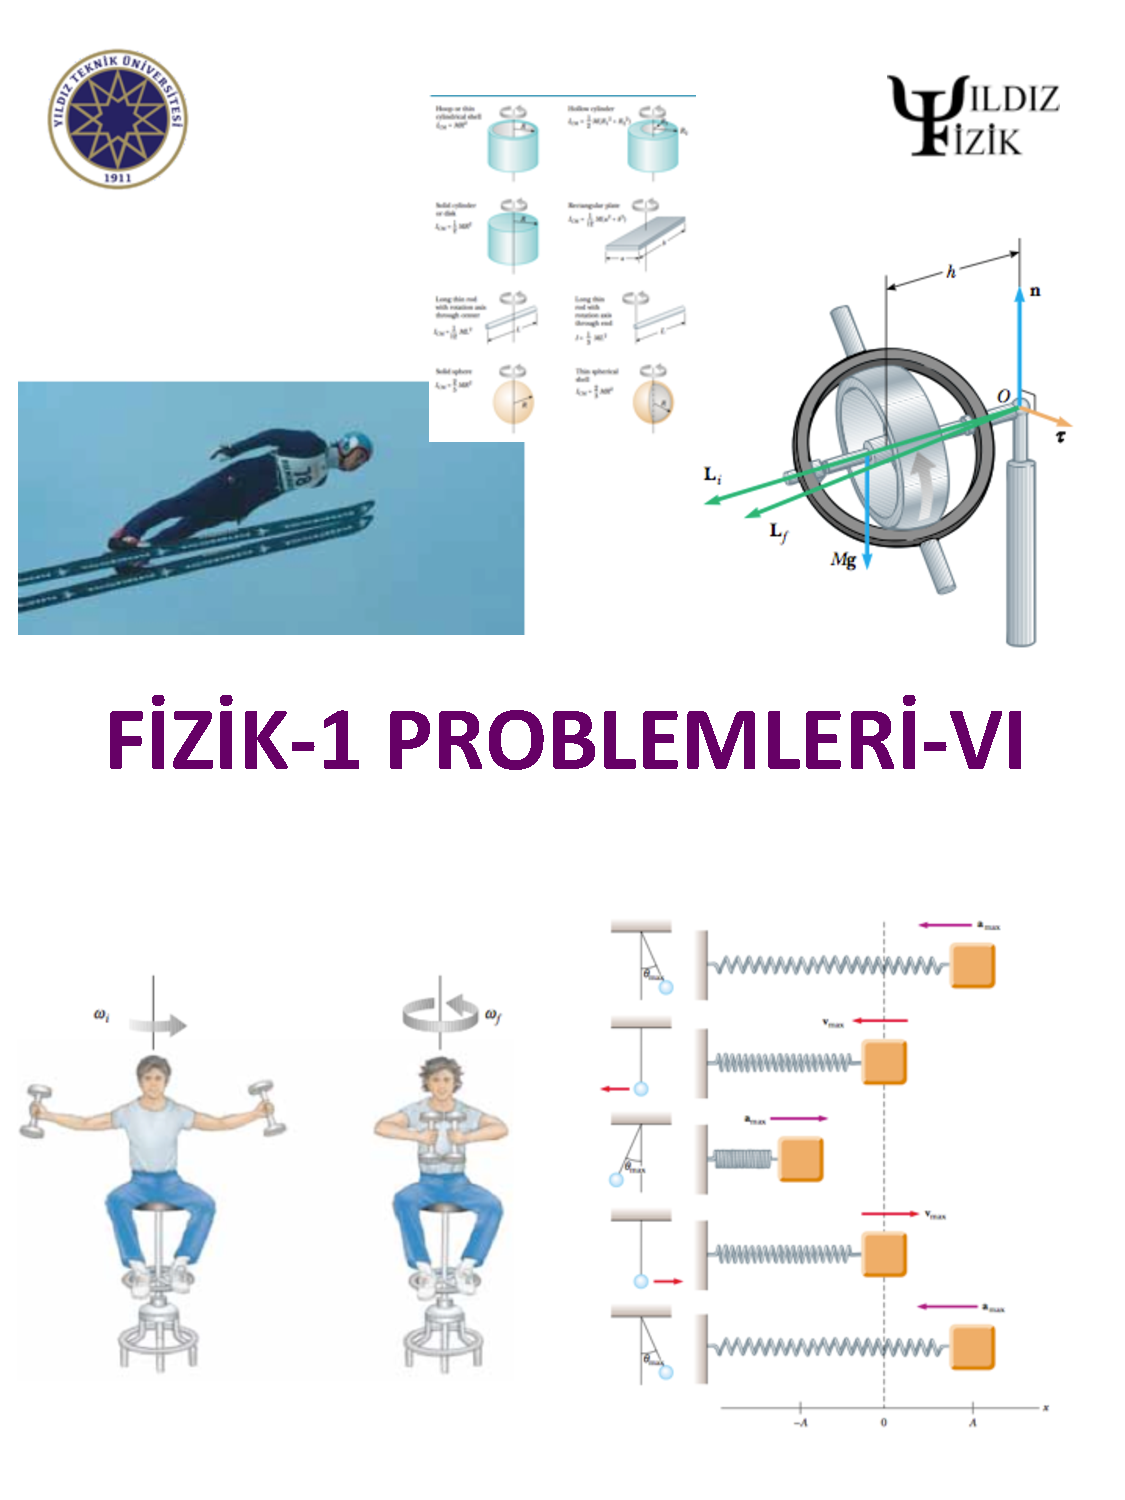
\includegraphics[width=14cm]{7.png}
\caption{input-2.txt'den Barry, Neill.}
\label{fig:figure3}
\end{figure}
\begin{figure}[H]
\centering
\includegraphics[width=14cm]{8.png}
\caption{input-2.txt'den Efroni, Yehuda.}
\label{fig:figure3}
\end{figure}







\end{document}